\documentclass{article}


\usepackage[utf8]{inputenc}		% for special characters
\usepackage[english]{babel}
%\usepackage[T1]{fontenc}		% for correct use of western european characterfonts
\usepackage{amsmath}
\usepackage{bm}
\usepackage{natbib}
\usepackage{amssymb}
\usepackage{bbm}

\usepackage{titling}


\usepackage{graphicx}


\usepackage{algorithm}
\usepackage{algpseudocode}
% \usepackage{algorithm}
% keine "End"-Statements in Algorithmen
\algtext*{EndWhile}
\algtext*{EndIf}
\algtext*{EndFor}
\algtext*{EndProcedure}
\algtext*{EndFunction}



\usepackage{listings}
\usepackage{color} %red, green, blue, yellow, cyan, magenta, black, white
\definecolor{mygreen}{RGB}{28,172,0} % color values Red, Green, Blue
\definecolor{mylilas}{RGB}{170,55,241}	
	
\lstset{language=Matlab,%
	%basicstyle=\color{red},
	breaklines=true,%
	%morekeywords={matlab2tikz},
	keywordstyle=\color{blue},%
	% morekeywords=[2]{1}, keywordstyle=[2]{\color{black}},
	identifierstyle=\color{black},%
	stringstyle=\color{mylilas},
	commentstyle=\color{mygreen},%
	showstringspaces=false,%without this there will be a symbol in the places where there is a space
	numbers=left,%
	numberstyle={\tiny \color{black}},% size of the numbers
	numbersep=9pt, % this defines how far the numbers are from the text
	%emph=[1]{for,end,break},emphstyle=[1]\color{blue}, %some words to emphasise
	%emph=[2]{word1,word2}, emphstyle=[2]{style},    
}



\newcommand{\norm}[1]{\left\lVert#1\right\rVert}


\setlength{\parskip}{\baselineskip}
%\setlength{\parindent}{0pt}%

%\setlength{\parindent}{2em}
%\setlength{\parskip}{1em}
%\renewcommand{\baselinestretch}{1.5}


\begin{document}

\title{Kernel Density Estimates and Mean-Shift Clustering}
\author{Jonas Spinner\thanks{jonas.spinner@student.kit.edu} \enspace -- 1927895\\
	Analytics and Statistics\\
	KIT -- Karlsruhe Institute of Technologie}
\date{\today}
\maketitle

\newpage

\tableofcontents

\newpage

\listoffigures

\listoftables

\listofalgorithms

\newpage


\begin{abstract}
	In this seminar paper we are describing and evaluating the mean shift algorithm. It is a nonparametric clustering method which does not depend on prior knowledge on the number and shape of the clusters.
	
	The clusters are defined by the modes of the data density and a iteration procedure is used to let a point converge to its cluster centroid. We introduce the kernel density estimate for estimating the data density and then derive the mean shift algorithm from it.
	
	After presenting the methods we also present different applications of the algorithm, mainly its use in image segmentation.
\end{abstract}

\section{Introduction}

In this seminar paper I am going to discuss the method of kernel density estimation (KDE) and it's use in the mean-shift clustering algorithm (MSC). Clustering is one of the main tasks in Machine-Learning and MSC has many applications, mainly in image segmentation. The mean-shift algorithm is an non-parametric approach which allows a wide range of data distributions without imposing prior knowledge.

The content of this seminar paper is mainly based on \cite{Comaniciu.2002}.

\textbf{History}

The mean shift algorithm was introduced in \cite{Fukunaga.1975} where also the term ``mean shift'' was established. \cite{Comaniciu.2002} and \cite{Comaniciu.2003} are responsible for a gain in interest for the algorithm. These publication popularized the use of the algorithm in image segmenation and tracking.


\textbf{Notation}

In this paper I'm going to use the following conventions. Bold symbols $\bm{x}$ denotes a vector. $\{ \bm{x}_i \}_{i=1}^n$ denotes $n$ samples $\bm{x}_i$, indexed by $i$. $d$ is the dimensionality of the samples. $K(\cdot)$ is a multivariate kernel function $\mathbb{R}^d \rightarrow \mathbb{R}$ and $k(\cdot)$ denotes a single variable kernel function $\mathbb{R} \rightarrow \mathbb{R}$.


\section{Kernel Density Estimation}

In this section we are going to introduce the kernel density estimate. It will be used in the derivation of the mean shift algorithm.

\begin{figure}
	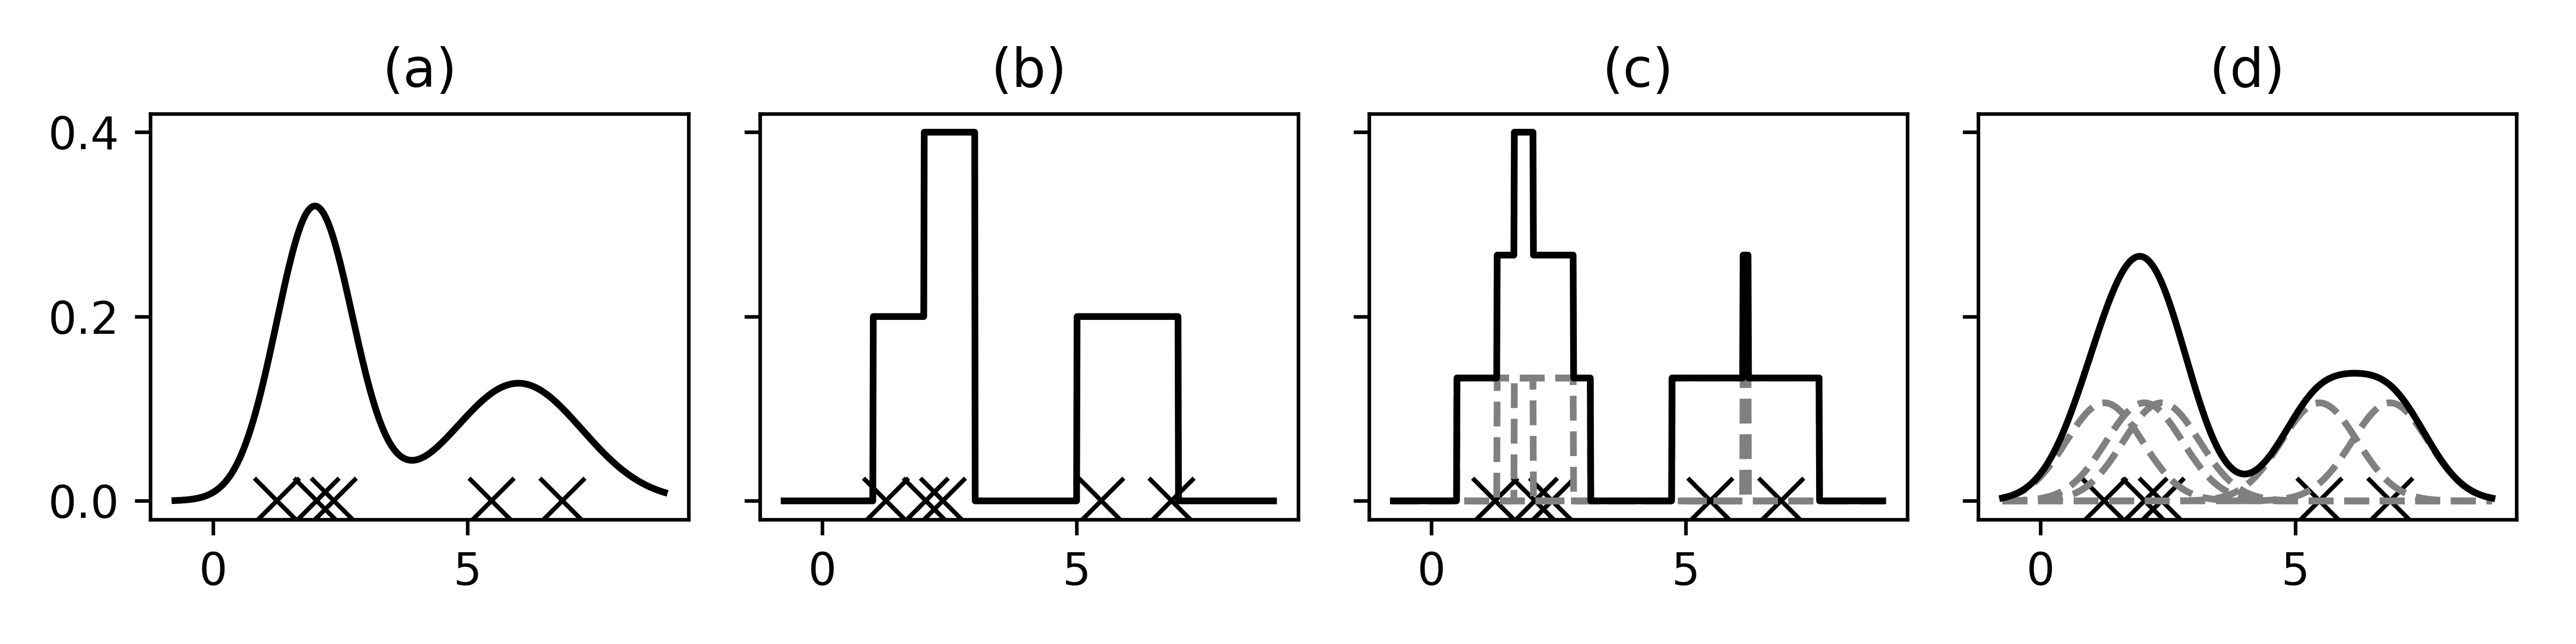
\includegraphics[width=\textwidth]{figures/kde-kernel-density-estimates}
	\caption[Samples, histogram and kernel density estimates]{Samples, histogram and kernel density estimates. Author's illustration.
		(a) The probability density distribution $p(x) = \frac{3}{5} N(x; 2, 0.75^2) + \frac{2}{5} N(x; 6, 1.25^2)$ and five samples drawn from it.
		(b) A histogram with bins $[i,i+1)$, $i \in \mathbb{Z}$.
		(c) A kernel density estimate with a uniform kernel and bandwidth $h=0.75$, $k(x) = \frac{1}{2h}$ for $\lvert x \rvert \leq h$ and $0$ else.
		(d) A kernel density estimate with a gaussian kernel and bandwidth $h=0.75$, $k(x) = \frac{1}{h} \frac{1}{\sqrt{2\pi}} \exp(-\frac{1}{2} \lvert \frac{x}{h} \rvert^2)$.
	}
	\label{fig:kde-kernel-density-estimates}
\end{figure}

% Some methods and algorithms require a probability density function (pdf) of the distribution but only samples are available.

We assume that we have $n$ data points $\{\bm{x}_i\}_{i=1}^n \subset \mathbb{R}^d$, which are independently, identically distributed samples from a unknown probabiltiy distribution $p(\bm{x})$, $\bm{x}_i \overset{i.i.d.}{\sim} p(\cdot)$. We call the corresponding density function $f$. 

The goal of density estimation is estimating the probality density of $p$, given samples $\{\bm{x}_i\}_{i=1}^n$ in $\mathbb{R}^d$, $\bm{x} \sim p(\bm{x})$.


Histograms estimate the probability distribution by bucketing the samples and counting the proportion of samples which fall in each bucket.

The \textbf{kernel density estimate} is defined as

\begin{equation}
	\hat{f}(\bm{x}) = \frac{1}{nh^d} \sum_{i=1}^n K\left(\frac{\bm{x} - \bm{x}_i}{h} \right) \qquad \bm{x} \in \mathbb{R}^d\text{,}
	\label{eq:kernel-density-estimate}
\end{equation}

where $n$ is the sample size, $d$ is the dimensionality of the data, $K(\bm{x})$ is a kernel function and $h$ is a bandwidth parameter. The estimate is dependent on the choice of the kernel function and the bandwidth.

A \textbf{kernel function} $K(\bm{x})$ is a function that satisfies $K(\bm{x}) \geq 0$ and $\int_{\mathbb{R}^d} K(\bm{x}) d\bm{x} =\nobreak 1$. These restrictions on the kernel ensure that $\hat{f}(\bm{x})$ is a valid density. The \textbf{bandwidth} $h$ controls the smoothness of the kernel density estimate. We are going to discuss the choices for kernel functions and the bandwidth in the next section.

The kernel density estimate can be interpreted as the sum of ``bumps'' centered on each data point.

For non-negative kernels, one can see that $\hat{f}(\bm{x})$ is a valid probability density.


\subsection{Other methods}

Another method for estimating a probability density function are histograms. The samples $\{ \bm{x}_i \}_{i=1}^n$ are put into distinct buckets $b_j \subseteq \mathbb{R}^d$ and the probability is estimated by the sample frequency $p(j) = \lvert \{\bm{x}_i \mid \bm{x}_i \in b_j\} / n$ for each bucket.


\subsection{Popular Kernels}

% Kernels:
% uniform, triangular, biweight, triweight, Epanechnikov, normal, and others

% Estimators:
% Nadaraya-Watson kernel-weighted average

\begin{figure}
	\centering
	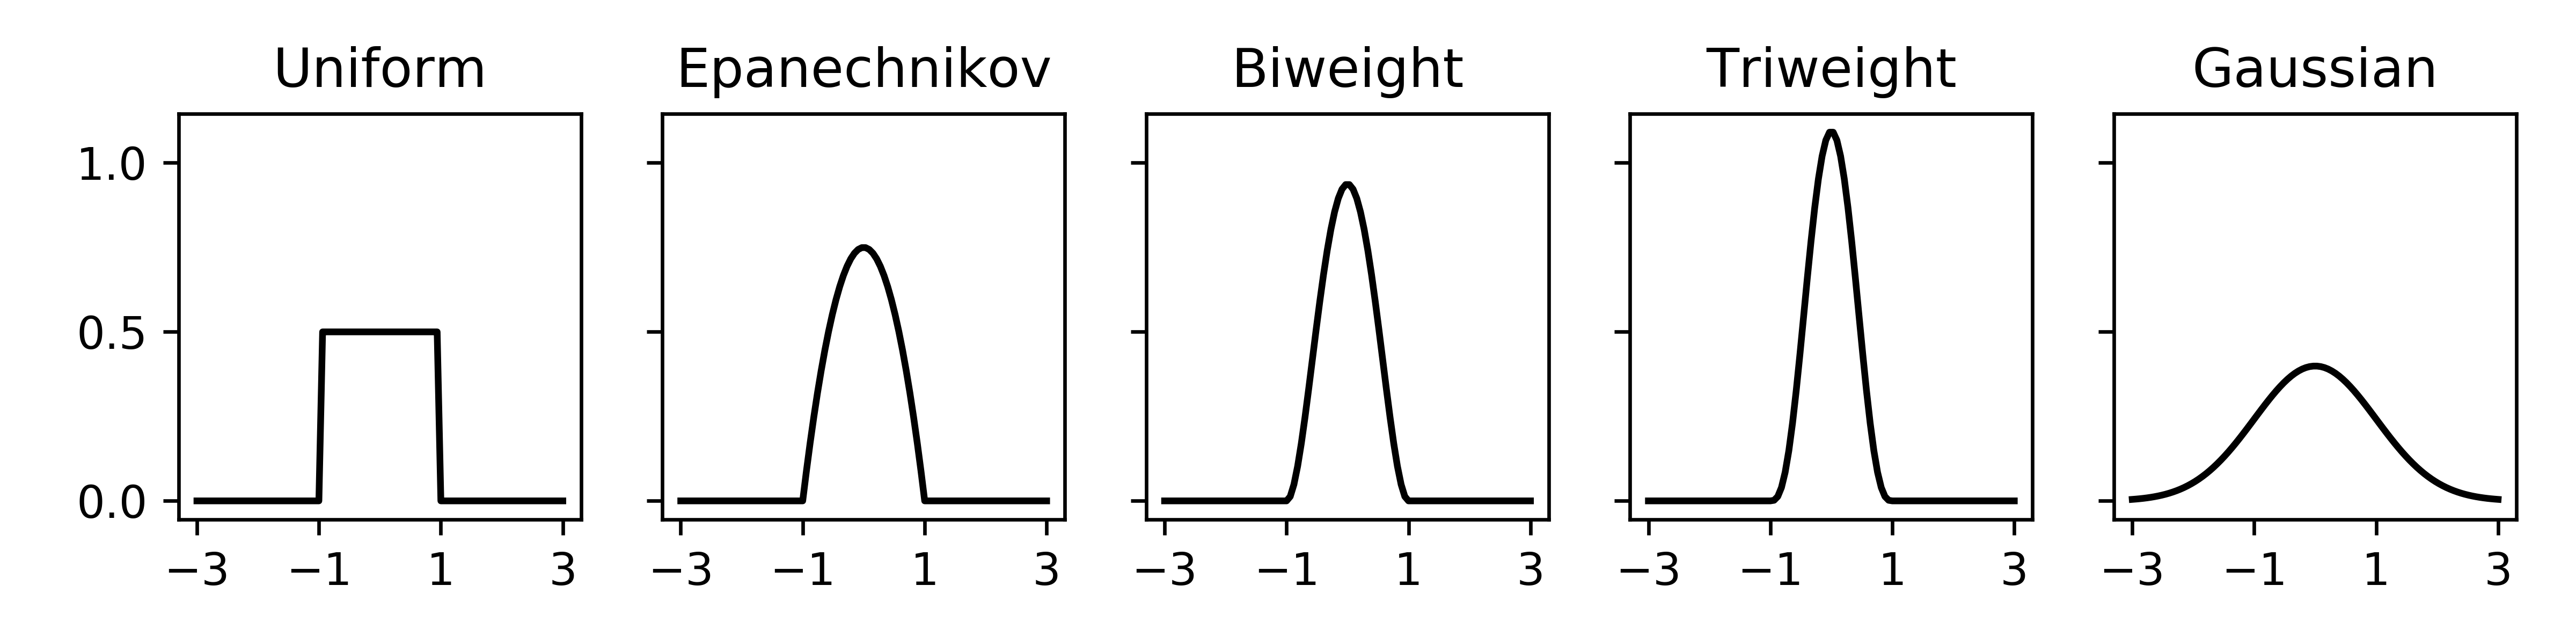
\includegraphics[width=\textwidth]{figures/kde-popular-kernels}
	\caption[Popular kernels]{Popular kernels. Author's illustration. The first four kernels all have support $[-1, 1]$. The gaussian kernel has the support $(-\infty, \infty)$.}
	\label{fig:kde-popular-kernels}
\end{figure}

A general Kernel is a function $K : \mathbb{R}^d \rightarrow \mathbb{R}$ satisfying the following properties. See \citep{Comaniciu.2002} and \citep[p.~95]{Wand.1995}.

\begin{align*}
	\int_{\mathbb{R}^d} K(\bm{x})\mathrm{d}\bm{x} &= 1 \qquad \int_{\mathbb{R}^d} \bm{x} K(\bm{x})\mathrm{d}\bm{x} = \bm{0} \\
	\lim_{\norm{\bm{x}} \rightarrow \infty}  \norm{\bm{x}}^d K(\bm{x})\mathrm{d}\bm{x} &= 0 \qquad \int_{\mathbb{R}^d} \bm{x} \bm{x}^T K(\bm{x})\mathrm{d}\bm{x} = c_K \bm{I}
\end{align*}

\begin{align*}
	K^P(\bm{x}) = \prod_{j=1}^d k(x_j) & \qquad
	K^S(\bm{x}) = a_{k,d} k(\norm{\bm{x}})
\end{align*}

Although there a many kernel functions, we are going to concentrate us on one class of functions: \textbf{radially symmetric kernels}. They are the kernels which can be formulated as

\begin{equation}
	K(\bm{x}) = c_{k,d} k(\norm{\bm{x}}^2)\text{,}
\end{equation}

where $k : [0, \infty]) \rightarrow [0, \infty)$ is called the \textbf{profile} of $K$, and $c_{k,d}$ is a constant which ensures, that $K(\bm{x})$ integrate to 1.

The derivation of the mean shift algorithm is going to be easier and nearly all popular kernels already belong to this class. The most popular kernels for mean shift clustering are the uniform, Epanechnikov and the Gaussian kernel. We are going to shortly introduce them and their profile.

The \textbf{uniform kernel} is defined as being constant in the unit hypersphere and can be written as
\begin{equation}
	K_U(\bm{x}) = \begin{cases}
		\text{vol}(S_d)^{-1} & \text{for} \norm{\bm{x}} \leq 1\\
		0 & \text{else}
	\end{cases}\text{,}
\end{equation}
where $\text{vol}(S_d) = \pi^{d/2}\Gamma((d+2)/2)^{-1}$ is the volume of the d-dimensional hypersphere. If $d=1$ then $\text{vol}(S_d)=2$. The corresponding profile $k_U$ is
\begin{equation}
	k_U(u) = \begin{cases}
		1 & \text{for } 0 \leq u \leq 1\\
		0 & \text{for } 1 < u\text{.}
	\end{cases}
\end{equation}

The \textbf{Epanechnikov kernel} is defined as
\begin{equation}
	K_E(\bm{x}) = \begin{cases}
		\frac{2 + d}{2 \text{vol}(S_d)} (1 - \norm{\bm{x}}^2) & \text{for } \norm{\bm{x}} \leq 1\\
		0 & \text{else}
	\end{cases}
\end{equation}
and its profile $k_E$ is
\begin{equation}
	k_E(u) = \begin{cases}
		1 - u & \text{for } 0 \leq u \leq 1\\
		0 & \text{for } 1 < u\text{.}
	\end{cases}
\end{equation}

The \textbf{gaussian kernel} is defined as
\begin{equation}
	K_G(\bm{x}) = (2 \pi)^{-d/2} \exp\left(-\frac{1}{2} \norm{\bm{x}}^2\right)
\end{equation}
and its profile $k_G$ is
\begin{equation}
	k_G(u) = \exp\left(-\frac{1}{2}u\right)\text{.}
\end{equation}



\begin{table}[]
	\centering
	\begin{tabular}{lll}
		\hline
		Name & Formula & Support \\ \hline
		Uniform & $k(x) = \frac{1}{2}$ & $[-1, 1]$ \\
		Epanechnikov & $k(x) = \frac{3}{4} (1 - x^2)$ & $[-1, 1]$ \\
		Biweight & $k(x) = \frac{15}{16} (1 - x^2)^2$ & $[-1, 1]$ \\
		Triweight & $k(x) = \frac{35}{32} (1 - x^2)$ & $[-1, 1]$ \\
		Gaussian & $k(x) = \frac{1}{\sqrt{2\pi}}\exp(-\frac{u^2}{2}) $ & $(-\infty, \infty)$
	\end{tabular}
	\caption{Popular kernels}
	\label{tab:popular-kernels}
\end{table}

\subsection{Bandwidth Selection}

One of the main challenges in using the kernel density estimator in practice is the choice of the bandwidth.


\section{Mean Shift Clustering}

Clustering is one of the main machine learning tasks, concerned with grouping objects $\{x_i\}_{i=1}^n$ into clusters $C_j$ resulting in a clustering $\{ C_j \}_{j=1}^K$.

\subsection{A general perspective on clustering algorithms}

\textit{introduction}

What does define a good clustering? One can try to minimize a global criterion like $J = \sum_{j=1}^K \sum_{\bm{x}_i \in C_j} \norm{\bm{x}_i - \bm{m}_j}^2$, like the $K$-Means algorithm, or minimize the intra-cluster min, max or average distances between the data points, like in hierarchical clustering. The notion of a ``good'' clustering brings rise to many different clustering algorithms.

Another criteria to differentiate clustering algorithms, are the assumptions that it makes on the data. $K$-Means assumes the data is separable into $K$ clusters. 

There are many different notions of what defines a good clustering and what shapes a cluster can take. These different notions result in different clustering algorithms. One class of clustering algorithms is centroid based clustering. Each cluster is represented by a representative called centroid. For example the representative of a $K$-Means clustering is the mean of the cluster $m_j := \frac{1}{\lvert C_j \rvert} \sum_{x_i \in C_j} x_i$.

\textit{centroid based}

A common concept for several algorithms are \textbf{centroids}. A centroid is a point in the data space, which is a representative for a cluster. $K$-Means defines its centroids as the cluster mean $\bm{m}_j = \frac{1}{\lvert C_j \rvert} \sum_{\bm{x}_i \in C_j} \bm{x}_i$. A shortcoming of this definition is that the cluster mean is not guaranteed to ``look like'' a typical data object.

The mean shift algorithm defines its cluster representatives by the modes of the data density. This definition solves several of shortcomings of other algorithms. The algorithm does not make prior assum


Another way clustering algorithms can be differentiated is whether of not the amount of clusters is given as an input to the algorithm or not. For example the $K$-Means algorithm searches for exactly $K$ clusters. But there are also other notions of a cluster center or representative. One is the added restriction, that the center is itself a data object or atleast ``looks like'' one. The latter is covered by using representatives which are likely also a data object. That's the core of the mean shift clustering algorithm. It estimates the underlying density of the data objects and searches for points which high relative probability. Or in other words it identifies the modes of the estimated density.

That leaves open on how to estimate the density.

\subsection{Density gradient estimation}

Before looking at the algorithm itself, we are going to derive the name giving mean shift vector by estimating the density gradient with the gradient of the density estimate. This subsection is based on \cite{Comaniciu.2002} and follows its notation.

As we have discussed in the previous subsection, one way to define a cluster is by the modes of the the density. This is notion that is the main point of this paper. The task is to find the points $\bm{x}$ where the density gradient vanishes, $\nabla f(\bm{x}) = 0$.

The density is estimated with kernel density estimation. Recall that the density estimate is formulated as

\begin{equation}
	\hat{f}(\bm{x}) = \frac{1}{nh^d} \sum_{i=1}^n K\left(\frac{\bm{x} - \bm{x}_i}{h} \right)\text{.}
	\label{eq:kernel-density-estimate-2}
\end{equation}

A natural way to estimate the density gradient is to use the gradient of the density estimate. Formally we write

\begin{equation}
	\hat\nabla f(\bm{x}) \equiv \nabla \hat{f}(\bm{x}) = \frac{1}{nh^d} \sum_{i=1}^n \nabla K\left(\frac{\bm{x} - \bm{x}_i}{h} \right)\text{.}
	\label{eq:kernel-density-gradient-estimate}
\end{equation}


To simplify the coming derivation we are going to concentrate on a class of kernels, \textbf{radially symmetric kernels}. These can be written as

\begin{equation}
	K(\bm{x}) = c_{k,d} k(\norm{\bm{x}}^2)
\end{equation}

where $k : [0, \infty]) \rightarrow [0, \infty)$ is called the \textbf{profile} of $K$, and $c_{k,d}$ is a constant which ensures that $K(\bm{x})$ integrate to $1$. The most common kernels belong to this class of functions.

Because we are going to use different kernel density estimates, we explicit state the used bandwidth $h$ and kernel $K$ as a subscript on the kernel density estimate $\hat{f}_{h,K}(\bm{x})$. The kernel density estimate can now be formulated as
\begin{equation}
	\hat{f}_{h,K}(\bm{x}) = \frac{c_{k,d}}{nh^d} \sum_{i=1}^n k\left(\norm{\frac{\bm{x} - \bm{x}_i}{h}}^2 \right)\text{,}
	\label{eq:kernel-density-estimate-radial-symetric}
\end{equation}
and its gradient is
\begin{equation}
	\nabla \hat{f}_{h,K}(\bm{x}) = \frac{2c_{k,d}}{nh^{d+2}} \sum_{i=1}^n (\bm{x} - \bm{x}_i)k'\left(\norm{\frac{\bm{x} - \bm{x}_i}{h}}^2 \right)\text{.}
	\label{eq:kernel-density-gradient-estimate-radial-symetric}
\end{equation}

With the substitution $g(u) = -k'(u)$ and reordering we can reformulate the gradient to
\begin{equation}
	\nabla \hat{f}_{h,K}(\bm{x}) = \frac{2c_{k,d}}{nh^{d+2}} \left[\sum_{i=1}^n g\left(\norm{\frac{\bm{x} - \bm{x}_i}{h}}^2 \right)\right] \left[\frac{\sum_{i=1}^n \bm{x}_i g\left(\norm{\frac{\bm{x} - \bm{x}_i}{h}}^2 \right)}{\sum_{i=1}^n g\left(\norm{\frac{\bm{x} - \bm{x}_i}{h}}^2 \right)} - \bm{x}\right]\text{.}
\end{equation}

The expression can be decomposed into several terms. The last term is called mean shift vector,
\begin{equation}
	\bm{m}(\bm{x}) = \frac{\sum_{i=1}^n \bm{x}_i g\left(\norm{\frac{\bm{x} - \bm{x}_i}{h}}^2 \right)}{\sum_{i=1}^n g\left(\norm{\frac{\bm{x} - \bm{x}_i}{h}}^2 \right)} - \bm{x}\text{.}
\end{equation}

The first two factors can be decomposed into a scaling factor and a kernel density estimate with the kernel $G(\bm{x}) = c_{g,d} g(\norm{\bm{x}}^2)$
\begin{align}
	\frac{2c_{k,d}}{nh^{d+2}} \left[\sum_{i=1}^n g\left(\norm{\frac{\bm{x} - \bm{x}_i}{h}}^2 \right)\right] &= \frac{2c_{k,d}}{h^2c_{g,d}} \left[\frac{c_{g,d}}{nh^d} \sum_{i=1}^n g\left(\norm{\frac{\bm{x} - \bm{x}_i}{h}}^2 \right) \right]\\
	&= \frac{2c_{k,d}}{h^2c_{g,d}} \hat{f}_{h,G}(\bm{x})\text{.}
\end{align}

With these equations we can reformulate the density gradient estimate $\nabla \hat{f}_{h,K}(\bm{x})$ into
\begin{equation}
	\nabla \hat{f}_{h,K}(\bm{x}) = \frac{2c_{k,d}}{h^2c_{g,d}} \hat{f}_{h,G}(\bm{x}) \bm{m}(\bm{x})\text{.}
\end{equation}

That allows us to write the mean shift vector as a normalized gradient of the kernel density estimate $\nabla \hat{f}_{h,K}(\bm{x})$
\begin{equation}
	\bm{m}(x) = \frac{h^2c_{g,d}}{2c_{k,d}} \frac{\nabla \hat{f}_{h,K}(\bm{x})}{\hat{f}_{h,G}(\bm{x})}
\end{equation}


\begin{align}
	\nabla \hat{f}_{h,K}(\bm{x}) &= \frac{2c_{k,d}}{nh^{d+2}} \sum_{i=1}^n (\bm{x}_i - \bm{x})g\left(\norm{\frac{\bm{x} - \bm{x}_i}{h}}^2 \right)\notag\\
	&= \frac{2c_{k,d}}{nh^{d+2}} \sum_{i=1}^n (\bm{x}_i - \bm{x}) w_i\notag\\
	&= \frac{2c_{k,d}}{nh^{d+2}} \sum_{i=1}^n \bm{x}_i w_i - \bm{x} \sum_{i=1}^n w_i\notag\\
	&= \frac{2c_{k,d}}{nh^{d+2}} \left[\sum_{i=1}^n w_i\right] \left[\frac{\sum_{i=1}^n \bm{x}_i w_i}{\sum_{i=1}^n w_i} - \bm{x}\right]\notag\\
	&= \frac{2c_{k,d}}{nh^{d+2}} \left[\sum_{i=1}^n g\left(\norm{\frac{\bm{x} - \bm{x}_i}{h}}^2 \right)\right] \left[\frac{\sum_{i=1}^n \bm{x}_i g\left(\norm{\frac{\bm{x} - \bm{x}_i}{h}}^2 \right)}{\sum_{i=1}^n g\left(\norm{\frac{\bm{x} - \bm{x}_i}{h}}^2 \right)} - \bm{x}\right]\notag\\
	&= \frac{2c_{k,d}}{h^2c_{g,d}} \left[\frac{c_{g,d}}{nh^d} \sum_{i=1}^n g\left(\norm{\frac{\bm{x} - \bm{x}_i}{h}}^2 \right) \right] \bm{m}(\bm{x})\notag\\
	&= \frac{2c_{k,d}}{h^2c_{g,d}} \hat{f}_{h,G}(\bm{x}) \bm{m}(\bm{x})\notag
\end{align}


\begin{equation}
	\bm{m}(x) = \frac{h^2c_{g,d}}{2c_{k,d}} \frac{\nabla \hat{f}_{h,K}(\bm{x})}{\hat{f}_{h,G}(\bm{x})}
\end{equation}

\begin{align}
	k_N(u) &= \exp\left(-\frac{1}{2}u\right)\\
	-k_N'(u) &= \frac{1}{2}\exp\left(-\frac{1}{2}u\right) \propto k(u)\\
	K_N(\bm{x}) &= (2\pi)^{-d/2} \exp\left(-\frac{1}{2}\norm{\bm{x}}^2\right)
\end{align}

\begin{align}
	k_E(u) &= \begin{cases}
		1 - u & 0 \leq u \leq 1 \\
		0 & 1 < u
	\end{cases}\\
	-k_E'(u) &= \begin{cases}
		1 & 0 \leq u \leq 1 \\
		0 & 1 < u
	\end{cases}\\
	K_E(\bm{x}) &= \begin{cases}
	\frac{1}{2} c_d^{-1} (d+2) (1 - \norm{\bm{x}}^2) & \norm{\bm{x}} \leq 1 \\
	0 & \text{else}
	\end{cases}
\end{align}

\begin{table}
	\begin{tabular}{lllll}
		Name & Support & $k(u)$ & $-k'(u)$ & $K(\bm{x})$ \\ \hline
		Epanechnikov & $[0, 1]$ & $1 - u$ & $1$ & $\frac{1}{2} c_d^{-1} (d+2) (1 - \norm{\bm{x}}^2)$\\
		Gaussian & $(-\infty, \infty)$ & $\exp\left(-\frac{1}{2}u\right)$ & $\frac{1}{2}\exp\left(-\frac{1}{2}u\right)$ & $(2\pi)^{-d/2} \exp\left(-\frac{1}{2}\norm{\bm{x}}^2\right)$\\
		&&&&
	\end{tabular}
\end{table}


\subsection{The algorithm}

The core of the mean shift algorithm is an iterative procedure which acts on a single point $\bm{x}^{(0)}$. For the given point the algorithm finds the corresponding mode of the kernel density estimate ($\hat\nabla f(\bm{x}) = \bm{0}$). Each iteration step the point moves in the direction of the steepest ascent. The iteration stops when the point has converged to a fixed point $\bm{x}^{(t+1)} = \bm{x}^{(t)}$. For the clustering of a dataset, the iteration procedure is performed on each point. The samples used for the kernel density estimate are still fixed to the original dataset.

A variant of the algorithm is the blurring mean shift algorithm. There the kernel density estimate is based on the data points from the previous iteration step.

\begin{equation}
	\bm{m}(\bm{x}) = \frac{\sum_{i=1}^n \bm{x}_i g(\norm{\frac{\bm{x} - \bm{x}_i}{h}}^2)}{\sum_{i=1}^n g(\norm{\frac{\bm{x} - \bm{x}_i^2}{h}})} - \bm{x}
\end{equation}


\begin{equation}
	\bm{x}^{(t+1)} = \bm{x}^{(t)} + \bm{m}(\bm{x}^{(t)})\text{,}\qquad t = 1, 2, ...
\end{equation}

%From wikipedia
%2.1	Connectivity-based clustering (hierarchical clustering)
%2.2	Centroid-based clustering
%2.3	Distribution-based clustering
%2.4	Density-based clustering

%\begin{algorithm}
%	\caption{Euclid’s algorithm}\label{euclid}
%	\begin{algorithmic}[1]
%		\Procedure{Euclid}{$a,b$}\Comment{The g.c.d. of a and b}
%		\State $r\gets a\bmod b$
%		\While{$r\not=0$}\Comment{We have the answer if r is 0}
%		\State $a\gets b$
%		\State $b\gets r$
%		\State $r\gets a\bmod b$
%		\EndWhile\label{euclidendwhile}
%		\State \textbf{return} $b$\Comment{The gcd is b}
%		\EndProcedure
%	\end{algorithmic}
%\end{algorithm}

\begin{algorithm}
	\begin{algorithmic}[1]
		\Function{MeanShift}{$\{\bm{x}_i\}_{i=1}^n \subset \mathbb{R}^d$, $h : \mathbb{R}^+$, $\varepsilon : \mathbb{R}^+$}
		\State $\bm{Z} = \bm{X} : \mathbb{R}^{d\times n}$
		\Repeat
		\State $\bm{W} = (\exp(-\frac{1}{2} \norm{(\bm{x}_i - \bm{x}_j) / h}^2))_{i,j = 1..n}$
		\State $\bm{D} = \text{diag}(\sum_i \bm{W}_{ij})$
		\State $\bm{Q} = \bm{W} \bm{D}^{-1} : \mathbb{R}^{n\times n}$
		\State $\bm{Z} = \bm{X} \bm{Q} : \mathbb{R}^{d\times n}$
		\Until{\text{stop}}
		\State \Return \Call{ConnectedComponents}{$\{\bm{z}_i\}_{i=1}^n, \varepsilon$}
		\EndFunction
	\end{algorithmic}
	\caption{Mean-shift algorithm in matrix form.}
	\label{alg:mean-shift-algorithm-matrix-form}
\end{algorithm}

\begin{algorithm}
	\begin{algorithmic}[1]
		\Function{MeanShift}{$\bm{x}_1, ..., \bm{x}_n : \mathbb{R}^d$, $h$, $\varepsilon$}
		\For{$i = 1..n$}
		\State $\bm{x}^{(1)} = \bm{x}_i$, $t=0$
		\Repeat
		\State $t = t + 1$
		\State $\forall n: p(i \mid \bm{x}^{(t)}) = \frac{\exp(-\frac{1}{2} \norm{(\bm{x}^{(t)} - \bm{x}_i) / h}^2)}{\sum_{j=1}^n \exp(-\frac{1}{2} \norm{(\bm{x}^{(t)} - \bm{x}_j) / h }^2)}$
		\State $\bm{x}^{(t+1)} = \sum_{i=1}^n p(i \mid \bm{x}^{(t)}) \bm{x}_i$
		\Until{$\norm{\bm{x}^{(t+1)} - \bm{x}^{(t)}} < tol$}
		\State $\bm{z}_i = \bm{x}^{(t+1)}$
		\EndFor
		\State \Return \Call{ConnectedComponents}{$\{\bm{z}_i\}_{i=1}^n, \varepsilon$}
		\EndFunction
	\end{algorithmic}
	\caption{Mean-shift algorithm in iterative form.}
	\label{alg:mean-shift-algorithm-iterative-form}
\end{algorithm}


\subsection{Discussion}

\textit{Problems}

\textit{Performance}

The algorithm inhabits several problems. Some of them are dependent on the domain and data, like the choice of bandwidth and kernel, others are regarding the performance.

Methods for speedup

\section{Application}

\textit{image segmentation}

The main application for the mean shift clustering is image segmentation. Although the raw image data in the RGB-colorspace (red, green, blue) can be used, it is often not disereable. A human percieves distances of colors differently than the RGB-colorspace indicates. For that reason the image is often transformed in a more suitable colorspace, for example the L*u*v*-colorspace.

Another aspect is the spatial coherence of the clusters in the image. Two pixels with the same color, but in widely different parts of the image would be put in the same cluster. That can be prevented by adding imagespace information to the pixels. 

\subsection{Experiments}

\textit{basic clustering task}

\textit{image segmentation -- details}

\textit{dataset description}

\cite{Alpert.2012}

\subsection{Evaluation and Comparison}

\section{Summary}

We introduced general kernel density estimates and presented popular choices for kernels. We classify the mean shift clustering algorithm by it's understanding of a cluster and derive the iteration step coming from the kernel density estimate. We present different applications of the algorithm, mainly classic clustering tasks and 


\bibliographystyle{agsm}
\bibliography{KDEaMSC}


\appendix


\section{Code}

\begin{lstlisting}
function [A, C] = mean_shift(X, kernel, epsilon)
    tol = 1e-3; max_iter = 1000;
	
    Z = X;
    for t = 1:max_iter        
        W = apply_kernel(X, Z, kernel);
        D = diag(sum(W, 1));
        Q = W * D^(-1);
        Z_next = X * Q;

        % stop criteria
        if (max(abs(Z_next - Z), [], 'all') < tol)
            break
        end
    	Z = Z_next;
    end

    [A, C] = connected_component(Z, epsilon);
end
\end{lstlisting}


\section{Notation}

Data

\[
n\qquad \text{vs.} \qquad N
\]

\[
x\qquad \text{vs.} \qquad \bm{x}
\]

\[
x_i\qquad \text{vs.} \qquad x^{(i)}
\]

Kernels

\[
\hat{f}(x)\qquad \text{vs.} \qquad \hat{p}(x)
\]

\[
\hat{f}_h(x) = \frac{1}{n} \sum_{i=1}^n K_h(x - x_i)
\]

\[
\hat{f}_h(x) = \frac{1}{nh} \sum_{i=1}^n K\biggl(\frac{x - x_i}{h}\biggr)\qquad \text{vs.} \qquad \hat{f}_h(x) = \frac{1}{nh} \sum_{i=1}^n K\left(\frac{x - x_i}{h}\right)
\]

Radial Kernel

\[
\hat{f}_h(\bm{x}) = \frac{1}{n} \sum_{i=1}^{n} K_h(\norm{\bm{x} -\bm{x}_i})
\]

Product Kernel

\[
\hat{f}_h(\bm{x}) = \frac{1}{n} \sum_{i=1}^{n} \prod_{j=1}^d K_{h_j}(\bm{x}_j -\bm{x}_{ij})\qquad \text{vs.} \qquad \hat{f}(\bm{x}) = \frac{1}{n} \sum_{i=1}^{n} \prod_{j=1}^d K_{h_j}(\bm{x}_j -\bm{x}_j^{(i)})
\]

\newpage
\section*{Statutory Declaration}

I hereby declare, that I have written this seminar paper with the title \textbf{\thetitle} by myself and have not used other sources without declaration.


\begin{tabular}{@{}p{2in}p{2.5in}@{}}
	Karlsruhe, \thedate & \hrulefill \\
	& Jonas Spinner
\end{tabular}


\end{document}